\documentclass[paper=a4, fontsize=12pt]{scrartcl}
\usepackage{graphicx}
\usepackage[protrusion=true,expansion=true]{microtype}
\usepackage{amsmath,amsfonts,amsthm}
\usepackage{fourier}
\usepackage[utf8]{inputenc}
\usepackage{amsmath}
\usepackage{amsfonts}
\usepackage{amssymb}
\usepackage[OT4]{fontenc}
\usepackage[polish]{babel}
\usepackage{epstopdf}
\usepackage{fancyhdr}
\usepackage{hyperref}
\usepackage{multicol}
\pagestyle{fancyplain}
\fancyhead{}	
\renewcommand{\headrulewidth}{1pt}
\renewcommand{\footrulewidth}{1pt}
\textheight = 700pt
\textwidth = 500pt
\hoffset =-30pt
\begin{document}
\begin{flushright}
21.04.2016 r.\\
dr Robert Bryl
\end{flushright}Paweł Grabiński\\
Rok 3, Fizyka teoretyczna\\[0.5cm]
{\huge \bf Spektroskopia masowa}
\section{Opis teoretyczny}
\subsection{Spektrometria mass}
Spektrometria masowa jest bardzo istotną metodą badania złożonych cząsteczek chemicznych. Dzięki bardzo dużej czułości wykorzystywaa jest w wielu dziedzinach takich jak fizyka atomowa, geochronologia i analiza chemiczna(szczególnie w kontekście biologicznym).
\subsubsection{Podstawy spektormetrii masowej}
Pierwszy etap spektrometrii polega na wytworzeniu jonów badanej substancji, np. przez bombardowanie elektronami.
\begin{align*}
M+e^-\rightarrow M^{+.}+2e^-
\end{align*}
Wyprodukowany jon ulega rozpadowi. Należy zaznaczyć, że mówimy o kationorodniku i nieparzystej liczbie elektronów. W takiej sytuacji mamy dwa możliwe scenariusze rozpadu. Na rodnik i kation parzystoelektronowy lub obejętną cząsteczkę i nowy kationorodnik. By móc dobrze prześledzić proces zachodzący musimy odpowiednio zapisywać oba rodzaje jonów.
\begin{align*}
M^{+.}\begin{array}{c c c c}
 \rightarrow& EE^+& + & R^. \\
 \rightarrow& OE^{+.}& + & N
\end{array}
\end{align*}
Gdzie $EE^+$ oznacza kation parzystoelektronowy, a $OE^{+.}$. $R^.$ to rodnik, a $N$ to cząsteczka.\\

Oba rodzaje jonów mają różne własności chemiczne. Produkty takiego rozpadu mogą ulegać dalszej fragmentyzacji.

Wszelkie produkty tych przemian filtrowane są względem masy i są zliczane. Możemy tak otrzymać widmo masowe cząstki.

Większość jonów będzie miała ładunek wypadkowy wynikający z utraty jednego elektronu, ale możliwe jest powstanie również jonów podwójnie, co może być później wykryte w zależności od stosunku masy do ładunku.\\

Podstawowy schemat spektrometru masowego to:
\begin{itemize}
	\item układ wprowadzania substancji, np. chromatograf gazowy
	\item źródło jonów(do jonizacji substancji)
	\item zespół analizatorów do rozdzielania powstałych jonów
	\item detektor
	\item system zbierania danych
\end{itemize}
\begin{figure}[h!]
	\centering
	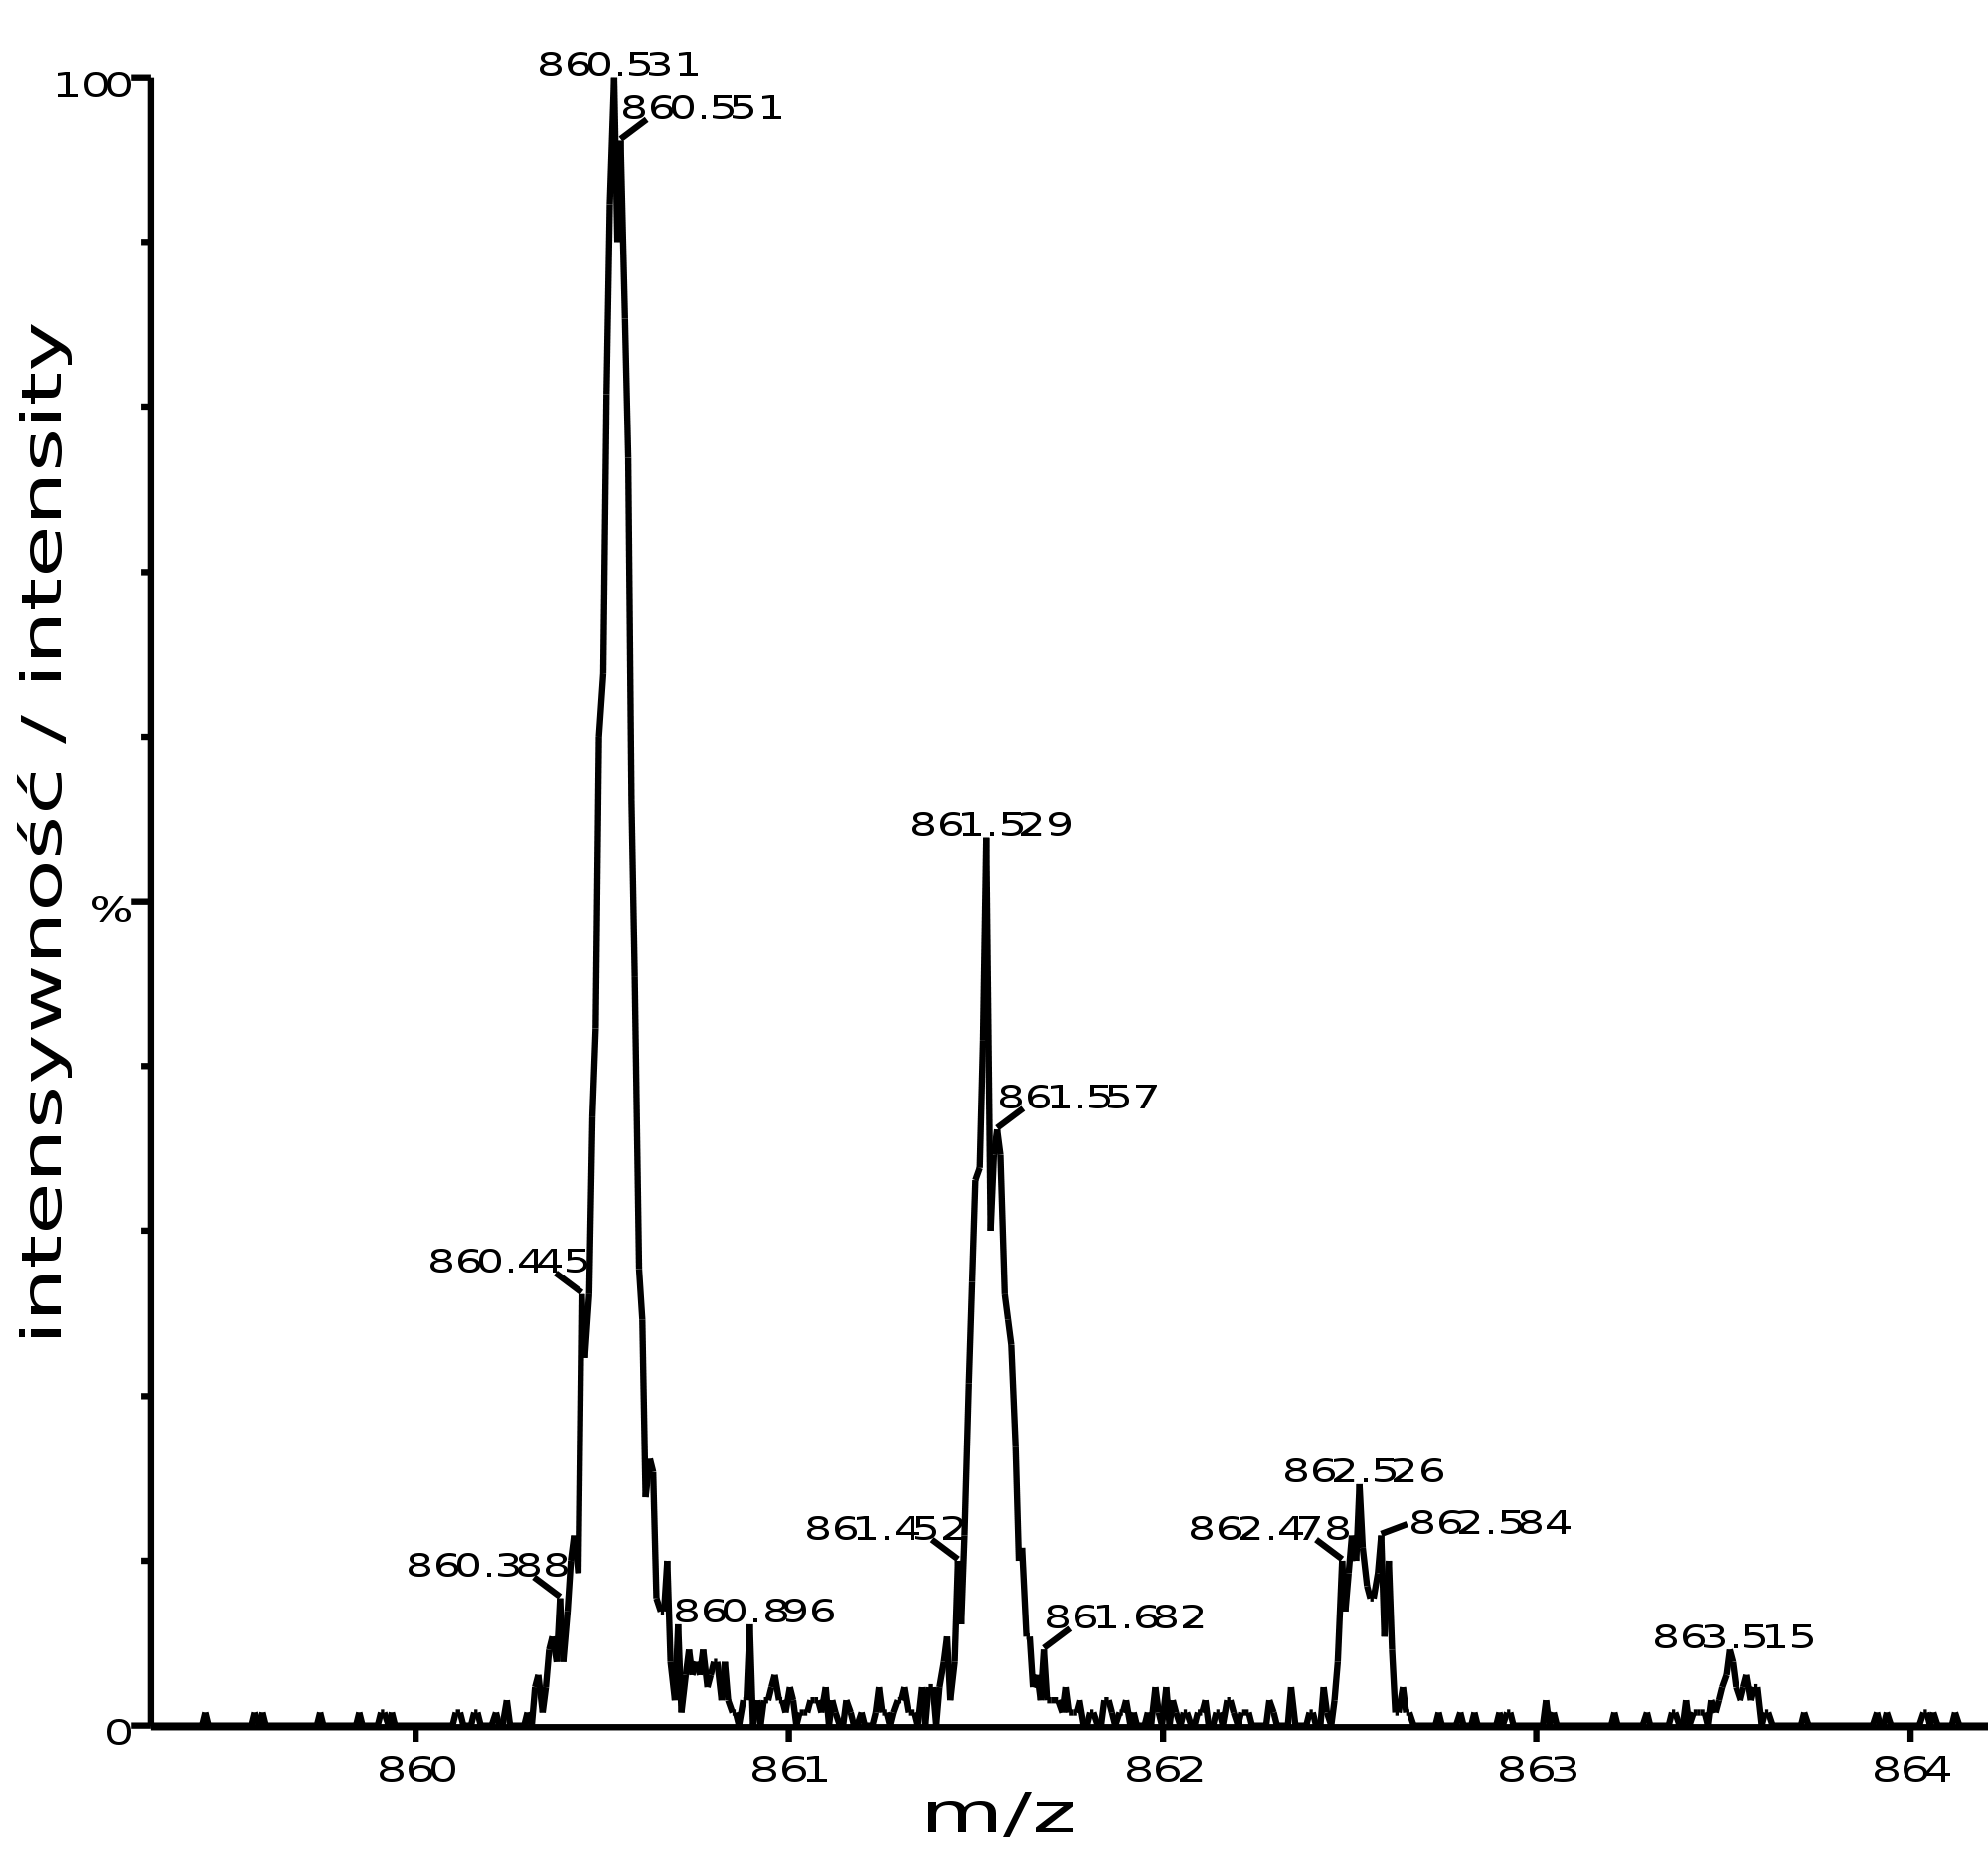
\includegraphics[width=0.5\linewidth]{mspek}
	\caption{Przykład widma masowego cząstki. Ostatnią linią spektrum będzie zjonizowana cząsteczka początkowa.}
	\label{fig:mspek}
\end{figure}
\subsubsection{Analizator kwadrupolowy}
Najważniejszą częścią spektroskopu masowego są analizatory oddzielające jony względem ich masy. Jednym z najczęściej stosowanych analizatorów jest analizator kwadrupolowy. Inne anzalizatory tego typu jak jonowa pułapka kwadrupolowa oraz analizator jonowego rezonansu cyklotronowego.
\begin{figure}[h!]
\centering
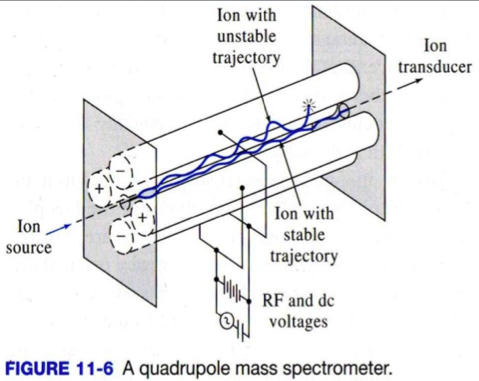
\includegraphics[width=0.48\linewidth]{quad}
\caption{Schemat analizator kwadrupolowego.}
\label{fig:quad}
\end{figure}\\
Analizator kwadrupolowy składa się z czterech prętów, mających w idealnym przypadku przekrój hiperboliczny. Zasada działania została opisana przez Paula i Steinwedela w 1953 r.
Dodatni jon przelatując przez obszar pomiędzy prętami jest przyciągany przez pręty o ujemnym potencjale. Jednak, gdy potencjał zmieni się na dodatni, to jon będzie odpychany i zmieni kierunek ruchu.\\
Pole elektryczne składa się z stałej składowej oraz składowej zmiennej w czasie.
\begin{align*}
\phi_0=(U-V\cos\omega t)\qquad -\phi_0=-(U-V\cos\omega t)
\end{align*}
Wartości napięcia $U$ to $500-2000\:\mathrm{V}$, a wartość $V$ to $0-3000\:\mathrm{V}$.
\subsubsection{Wielokrotny kwadrupol}
Łącząc szeregowo kwadrupole możemy uzyskać układ pomiarowy, w którym wprowadzana substancja będzie zderzać się z gazem kolizyjnym znajdującym się w jednym z połączonych kwadrupoli. Cząsteczka może ulec pojedynczemu lub wielokrotnym zderzeniom.\\

Jeśli gaz kolizyjny jest chemicznie nieczynny, to odbierze on energię od jonu, przekształcając częśc energii zderzenia w energię wewnętrzną. Jon ulegnie fragmentaryzacji, a jego składowe będą badane w dalszych kwadrupolach.\\

Jeśli gaz kolizyjny jest reaktywny, to będzie on powodował reakcję jon-cząsteczka, których produkty będą badane w dalszych kwadrupolach.
\subsubsection{Analizator unipolowy}
Podobną w działaniu konstrukcją jest analizator unipolowy. W porównianiu do kwadrupola, zamieniono w nim 3 pręty na metalową uziemioną "rynienkę" umieszczoną równolegle do pręta. Symuluje ona linie zerowego potencjału tworzące się w kwadrupolu. Zasada działania analogiczna do kwadrupolu. Jedyne różnice, to tylko jeden kierunek zakrzywiania toru cząstek oraz o połowę mniejsza odległość na jakiej może dochodzić do zakrzywień toru cząstki.
\subsection{Technika próżni}
By uzyskać jak najdokładniejsze wyniki pomiarowe, należy usunąć jak najwięcej czynników zakłócających. Jednym z tych czynników mogą być gazy oddziałujące z naszym układem. By zapobiec tego rodzaju problemom, rozwinięto wiele technologii umożliwiających wytowrzenie i utrzymanie próźni.\\
Technologie te stoją przed dwoma problemami, oceny oraz zmniejszenia ciśnienia w układzie.

\subsection{Pompy próżniowe}
Istnieje wiele rodzajów pomp próżniowych o wielu zasadach działania. Jedno przygotowują niską próżnię, czasem zwaną wstępną. Inne są w stanie wytworzyć bardzo wysoką próżnię.
\subsubsection{Pompa rotacyjna}
Składa się z cylindra, w którym znajduje się mimośrodowo ułożyskowany wirnik. W wielu szczelinach  wirnika są rozmieszczone łopatki, które przy obrocie wirnika dzięki sile odśrodkowej swoimi zewnętrznymi krawędziami ślizgają się wzdłuż wewnętrznej powierzchni cylindra. W ten sposób tworzy się pomiędzy dwoma łopatkami przestrzeń tłoczenia, której objętość w trakcie obrotu ciągle się zmienia. Poprzez kanał dolotowy powietrze wpływa do komory tłoczenia tak długo, aż tylna łopatka nie zamknie wejścia do kanału. Jeżeli teraz komora ssawna oddala się coraz bardziej od kanału zasysania, jej objętość staje się coraz mniejsza. Powietrze zamknięte w tej przestrzeni ulega sprężeniu i ciśnienie rośnie. Sprężanie trwa tak długo, aż ciśnienie w komorze sprężania przekroczy ciśnienie komory ciśnieniowej. Powietrze wypływa z komory poprzez kanał ciśnieniowy.
\begin{figure}[h!]
\centering
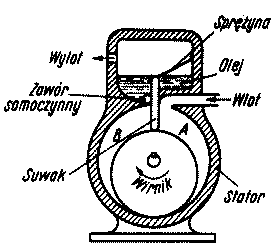
\includegraphics[width=0.4\linewidth]{rot2}
\caption{Schemat budowy pompy rotacyjnej.}
\label{fig:rot2}
\end{figure}

\subsubsection{Pompa turbomolekularna}
Podstawowymi elementami są dwa układy łopatek nieruchomego statora oraz obracającego się wirnika. Łopatki wirnika rozmieszczone są promieniście na osi, a łopatki statora na zewnętrznej obudowie. Płaszczyzna łopatek nie jest prostopadła do osi, lecz skręcona o pewien kąt. 
Wirnik wprawiany jest w ruch obrotowy, nadając cząsteczkom powietrza prędkość, tak że poruszają się one w kierunku wylotu pompy. W ten sposób cząsteczki są usuwane z wnętrza komory próżniowej i ciśnienie wewnątrz komory spada. Wirnik pompy obraca się bardzo szybko, tak by prędkość łopatek była porównywalna z prędkością ruchów cieplnych cząsteczek (ok. $ 10^3\ m/s$). Prędkość obrotowa może dochodzić do stu tysięcy obrotów na minutę. Wymaga próżni wstępnej rzędu $1\:\mathrm{Pa}$. Pompa turbomolekularna umożliwia wytworzeniu próżni $10^{-7}\:\mathrm{Pa}$.
\begin{figure}[h!]
\centering
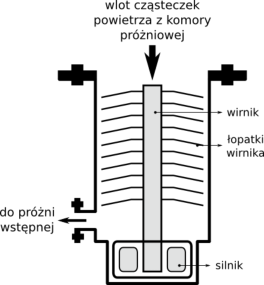
\includegraphics[width=0.5\linewidth]{turbo2}
\caption{Schemat budowy turbomlekularnej.}
\label{fig:turbo2}
\end{figure}

\subsubsection{Pompa jonowo-sorpcyjna}
Rodzaj pompy bezwylotowej. W pompie tej zachodzi jonizacja pompowanego gazu, do czego potrzebne jest duże przyłożone napięcie oraz opcjonalnie pole magnetyczne(przy niskich ciśnieniach, w celu usprawnienia jonizacji). Zjonizowany gaz uderzając w tytanową katodę, powoduje rozpylenie metalu, który osiada na ścianach układu. Reaktywne związki łączą sie z metalem, a gazy szlachetne są otaczane warstwą, która je "zabudowuje" na powierzchni ściany. Pompa ta wymaga próżni wstępnej $10^{-3}\:\mathrm{Tr}$. Za pomocą pompy jonowo-sorpcyjnej można uzyskać próżnię rzędu $10^{-11}\:\mathrm{Tr}$. Pompa ta daje czystą próżnię bez zanieczyszczeń olejem lub rtęcią.
\subsection{Próżniomierz Bayarda-Alperta}\begin{figure}[h!]
	\centering
	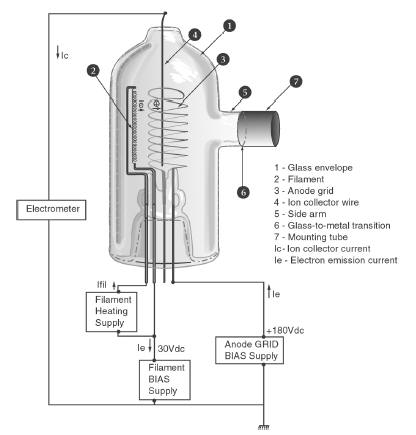
\includegraphics[width=0.4\linewidth]{BayardAlp}
	\caption{Schemat budowy głowicy Bayarda-Alperta.}
	\label{fig:BayardAlp}
\end{figure}
Budowa głowicy Bayarda-Alperta jest następująca, w próżniowej komorze połączonej z komorą pomiarową mamy trzy elementy:
\begin{itemize}
	\item Kolektor($4$) - prosty drut, na którym możemy mierzyć przepływ prądu i do którego przykładamy ujemny potencjał,
	\item Anoda($3$) - siatka lub zwój umieszczony symetrycznie dookoła kolektora, do której przykładamy dodatni potencjał,
	\item Katoda(katody)($2$) - drut wolfrwmowy, produkuje elektrony
\end{itemize}
Elektrony emitowane przez katodę przyspieszane są w potencjale anody i wpadają w obszar anody, gdzie jonizują znajdujące się tam atomy. Dodatnie jony atomów przyciągane są przez kolektor. W ten sposób możemy obserwować prąd przepływający na kolektorze.
\subsubsection{Problem lokalności próżni}
Jak widać z budowy próżniomierza Bayarda-Alperta, mierzy on tylko jakoś próżni w obrębie anody. Prowadzi to do dwóch problemów. Pierwszy i prosty, to opóźnienia w pomiarach związane z dochodzeniem do równowagi termodynamicznej układu. Drugi to fakt, że w trakcie pomiarów na anodzie mogą osadzać się badane gazy. Po ponowym włączeniu aparatury, gazy te moga zostać odparowane w wyniku bombardowania wysoko energetycznymi elektronami. W tym celu w wielu głowicach tego typu mamy dwie katody, które włączone równocześnie służą jej odgazowaniu.

\subsection{Spektrometr mas jako analizator gazów resztkowych}
Idealna próżnia nie jest możliwa do wytworzenia. W obrębie układu pomiarowego pozostaje wciąż pewna ilość gazów. Głównie wodór, który może dyfundować przez ściany aparatury. 
Dzięki analizatorowi masowemu, możemy określić jakie czasteczki składają się na nasz gaz resztkowy.
\section{Przebieg doświadczenia}
Aparatura pomiarowa udostępniona do ćwiczenia daje dostęp do dwóch trybów pomiarowych analizatora unipolowego:
\begin{itemize}
	\item Pomiar całego spektrum masowego
	\item Pomiar koncentracji gazu dla danej masy
\end{itemize}
Poza tym mamy do dyspozycji głowicę Bayarda-Alperta oraz źródło tlenu.
\subsection{Pomiary}
W ramach ćwiczenia wykonane zostały następujące pomiary:
\begin{enumerate}
	\item spektrum masowego gazów resztkowych dla różnych parametrów,
	\item koncentracji wodoru w trybie zależności czasowej z włączeniem głowicy Bayarda-Alperta,
	\item spektrum masowego przy włączonej głowicy,
	\item koncentracji tlenu w trybie zależności czasowej przy włączonym źródle(wyłączona głowica) do czasu stabilizacji,
	\item spektrum masowego ustabilizowanego układu.
\end{enumerate}
\clearpage
\section{Analiza pomiarów}
\subsection{Optymale parametry pomiarów}
Najlepsza rezultaty otrzymaliśmy dla następujących parametrów:
\begin{itemize}
	\item Time delay - $0.05\:\mathrm{s}$
	\item Time step - $0.05\:\mathrm{s}$
	\item $dm=0.001\:\mathrm{j.a.}$
	\item $m\:start=0\:\mathrm{j.a.}$
	\item $m\:end=45\:\mathrm{j.a.}$
	\item $U=0.0125\:\mathrm{V}$
\end{itemize}
Wyższe wartości Time delay oraz Time step nie polepszały istotnie otrzymywanych wyników, a niepotrzebnie zwiększały czas pomiarów. Mniejsze wartości tych parametrów prowadziły do dużego szumu spowodowanego efektami elektrostatycznymi.
\subsection{Początkowe spektrum masowe}
W początkowym spektrum widzimy głównie występowanie wodoru, tlenu, tlenku wodoru, wody i tlenku węgla.
\begin{figure}[h!]
	\centering
	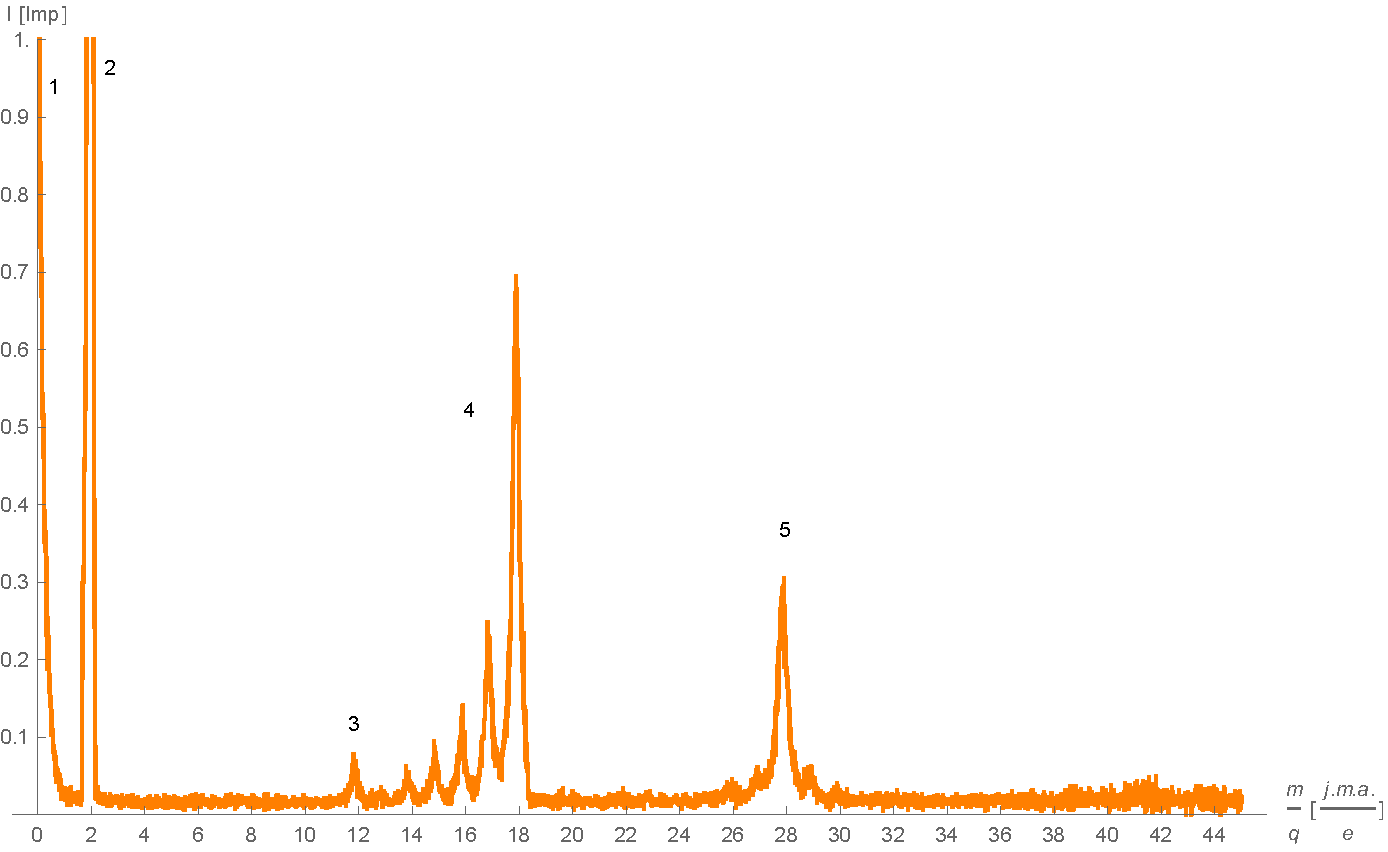
\includegraphics[width=0.7\linewidth]{spekini}
	\caption{Początkowe spektrum masowe gazów resztkowych znajdujących się w układzie.\newline 1 - peak elektrostatyczny; 2 - wodór(2); 3 - węgiel(12); 4 - odpowiednio tlen(16),\newline tlenek wodoru(17) i woda(18); 5 - tlenek węgla(28).}
	\label{fig:spekini}
\end{figure}\\
\newpage
\subsection{Rozdzielczość analizatora}
By wyznaczyć rozdzielczość, dokonano cięcia na $I=0.023$. Dalej odczytano szerokość maksimów w połowie ich wysokości względem danego cięcia.
\begin{figure}[h!]
\centering
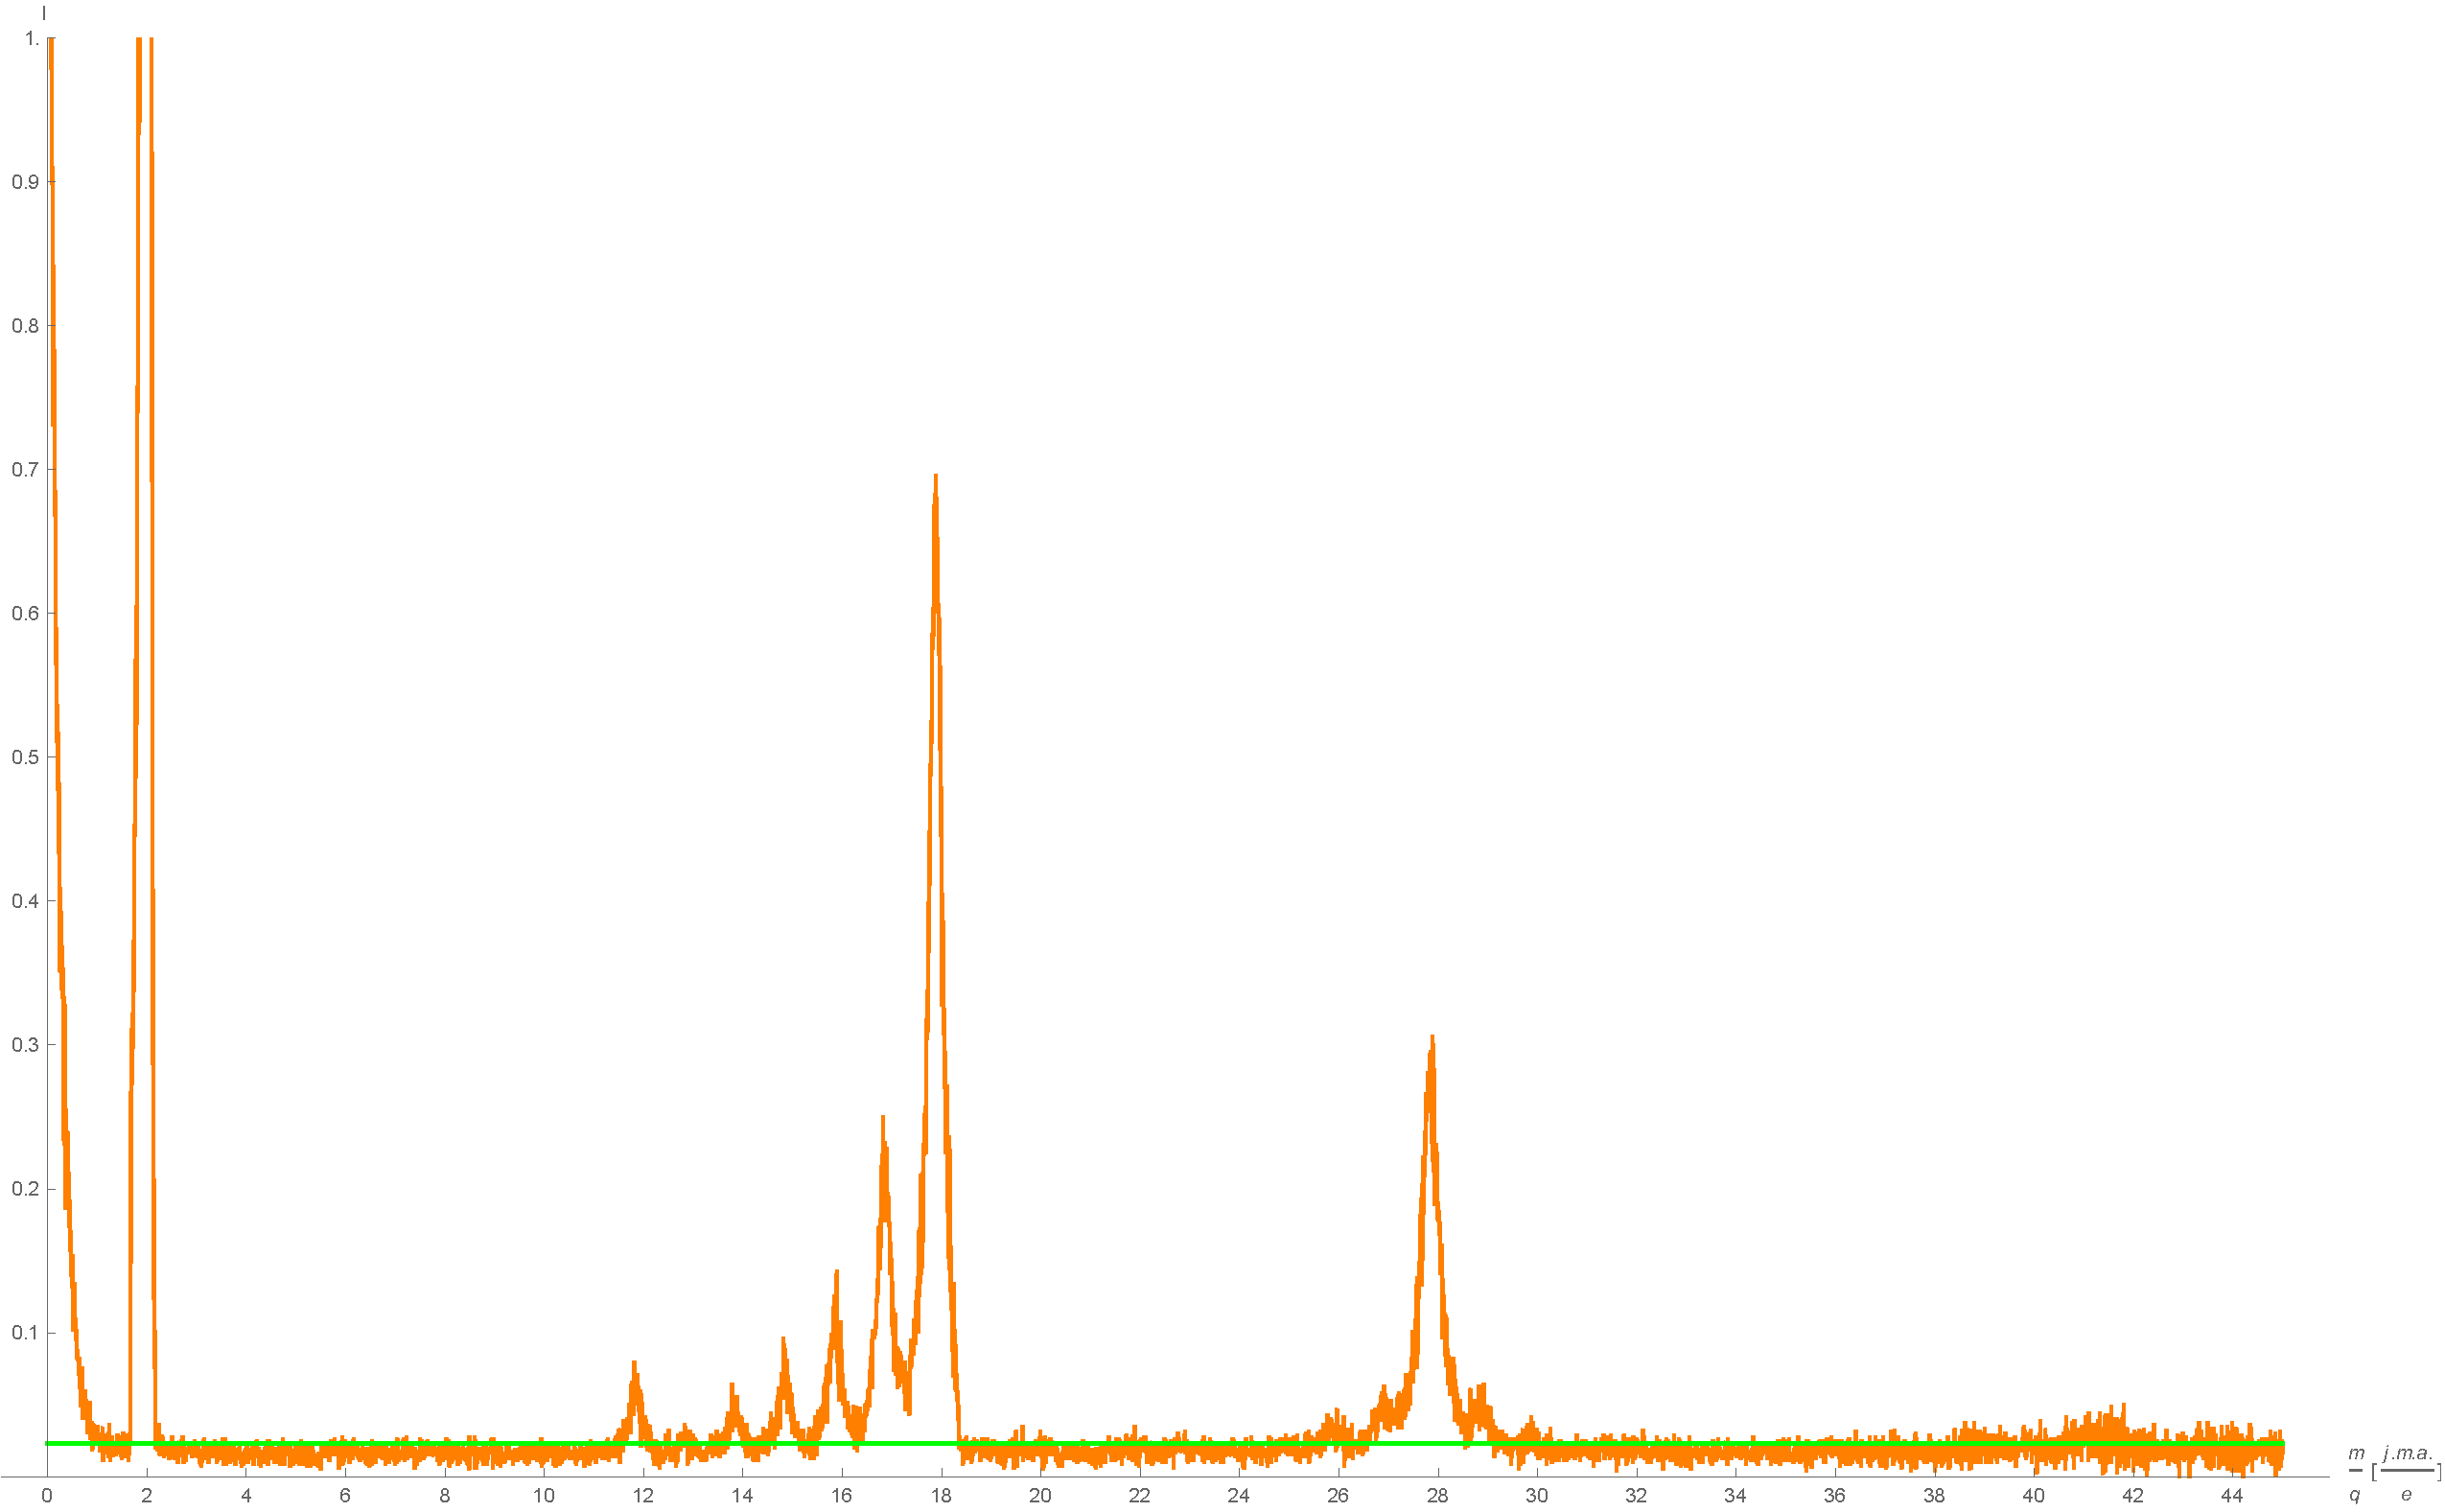
\includegraphics[width=0.7\linewidth]{spektcut}
\caption{Spektrum wraz z cięciem jakie zostało dokonane dla wybrania maksimów.}
\label{fig:spektcut}
\end{figure}\\
Otrzymaliśmy następujące szerokości dla kolejnych maksimów.
\begin{table}[h!]
	\begin{tabular}{|c|c|c|c|c|c|c|c|c|}\hline
$d\alpha_i$ & 0.14 & 0.55 & 0.59 & 0.34 & 0.33 & 0.39 & 0.3 & 0.43 \\\hline 
\end{tabular}
\end{table}\\
Licząc średnią tych rozpiętości dostajemy, że rozdzielczość analizatora wynosi $d\alpha=0.38375\:\mathrm{j.a.}$

\subsection{Koncentracja wodoru w trakcie pracy głowicy Bayarda-Alperta}
\begin{figure}[h!]
\centering
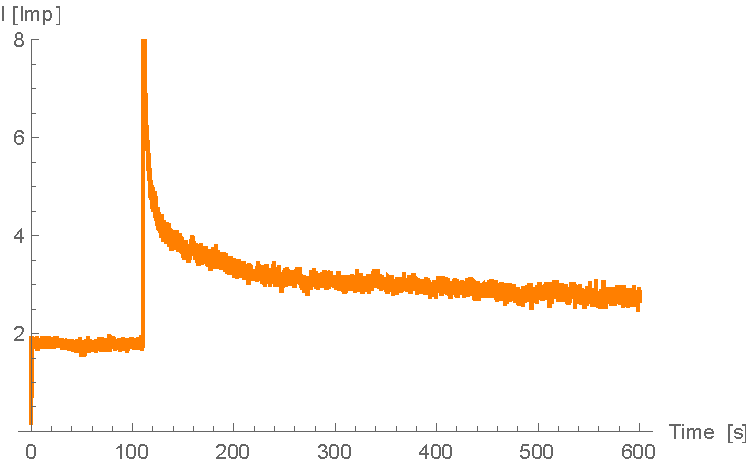
\includegraphics[width=0.5\linewidth]{hydtime}
\caption{Zmiana w czasie koncentracji wodoru. Widoczy skok w momencie włączenia głowicy Bayarda-Alperta i późniejszy bardzo powolny spadek w kieruku uprzedniego poziomu.}
\label{fig:hydtime}
\end{figure}
\subsection{Spektrum masowe w trakcie pracy głowicy Bayarda-Alperta}
Widzimy, że włączenie głowicy Bayarda-Alperta spowodowało zwiększenie koncentracji związków występujących w układzie pomiarowym. Wynika to z budowy głowicy B-A, która na początku swojej pracy odgazowuje się i zwiększa ciśnienie w układzie pomiarowym. \\
\begin{figure}[h!]
\centering
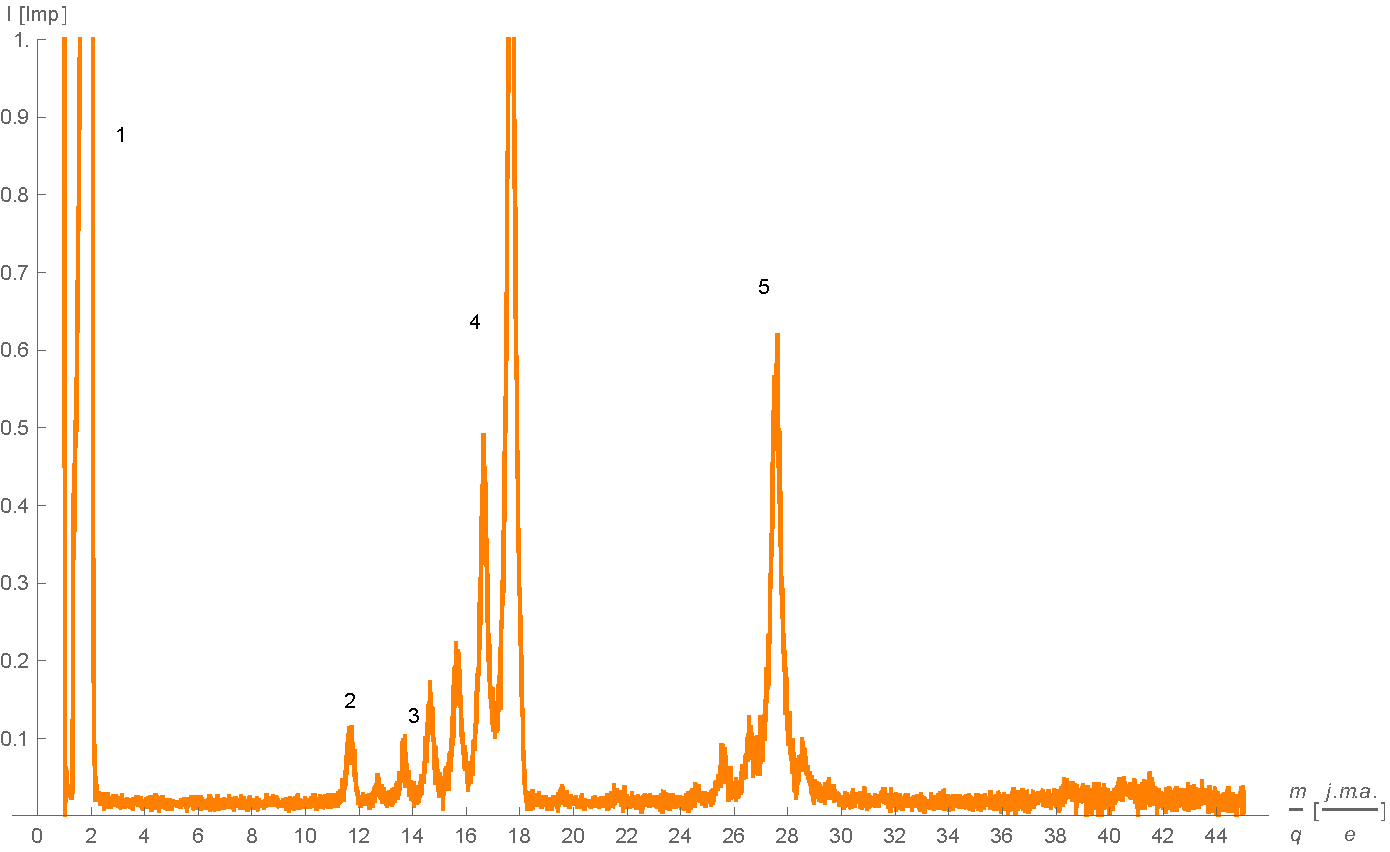
\includegraphics[width=0.7\linewidth]{spekba}
\caption{Spektrum masowe przy włączonej głowicy Bayarda-Alperta.\newline 1 - peak elektrostatyczny(0-1) oraz wodór(2); 2 - węgiel(12); 4 - odpowiednio tlen(16),\newline tlenek wodoru(17) i woda(18); 5 - tlenek węgla(28).}
\label{fig:spekba}
\end{figure}\\
Na uwagę zasługują maksima oznaczone numerem $3$ odpowiadające liczbom $13$, $14$ i $15$, które wcześniej zostały zaniedbane. Liczba $13$ odpowiada jonom $CH$. Jednak liczba $14$ jest trudniejsza do zidentyfikowania. Może to być zarówno $CH_2$(grupa metylenowa) jak i $N$(azot). O ile grupy metylenowej nie jesteśmy w stanie zidentyfikować, to możemy szukać cząstek $N_2$. Jednak ich masa jest taka samoa jak masa tlenku węgla, więc nie możemy wnioskować na podstawie tego. Pewną wskazówkę daje nam kolejne maksimum dla liczby $15$. Ponieważ trójtlenek węgla jest związkiem niestabilnym, spodziewamy się, że będzie to jon $NH$. Istotnie może to powierdzić także brak zaobserwowanych wcześniej jonów $CH$ odpowiadających liczbie $13$, przy istotnym odczycie dla liczb $14$ i $15$. Podsumowując, maksima odpowiadające liczbom wykazują obecność:
\begin{itemize}
	\item $13$ - jony $CH$
	\item $14$ - azot $N$
	\item $15$ - jony $NH$
\end{itemize}
\newpage
\subsection{Koncentracja tlenu przy włącząnym źródle tlenu}
Źródło tlenu włączone zostało około $100$. sekundy. Jak widać poziom koncentracji ma dużą bezwładność w przypadku tego układu. Możemy zaobserwować maksimum po którym poziom spada. Spowodowane jest to tym, że sprawność pompy jonowo sorpcyjnej jest proporcjonalna do ilości gazu w układzie. Gdy gaz dociera w obszar pompy, zaczyna ona odpompowywać więcej gazu, dzięki czemu prędkość doprowadzania gazu i odprowadzania są na jednym poziomie. Co prowadzi do równowagi w układzie.
\begin{figure}[h!]
\centering
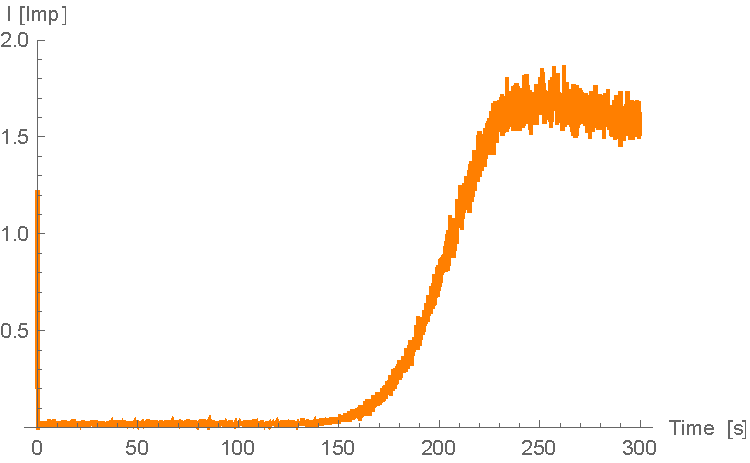
\includegraphics[width=0.6\linewidth]{32time}
\caption{Koncentracja tlenu przed i po włączeniu źródła tlenu}
\label{fig:32time}
\end{figure}\\


\subsection{Spektrum masowe po doprowadzeniu tlenu do układu}
\begin{figure}[h!]
\centering
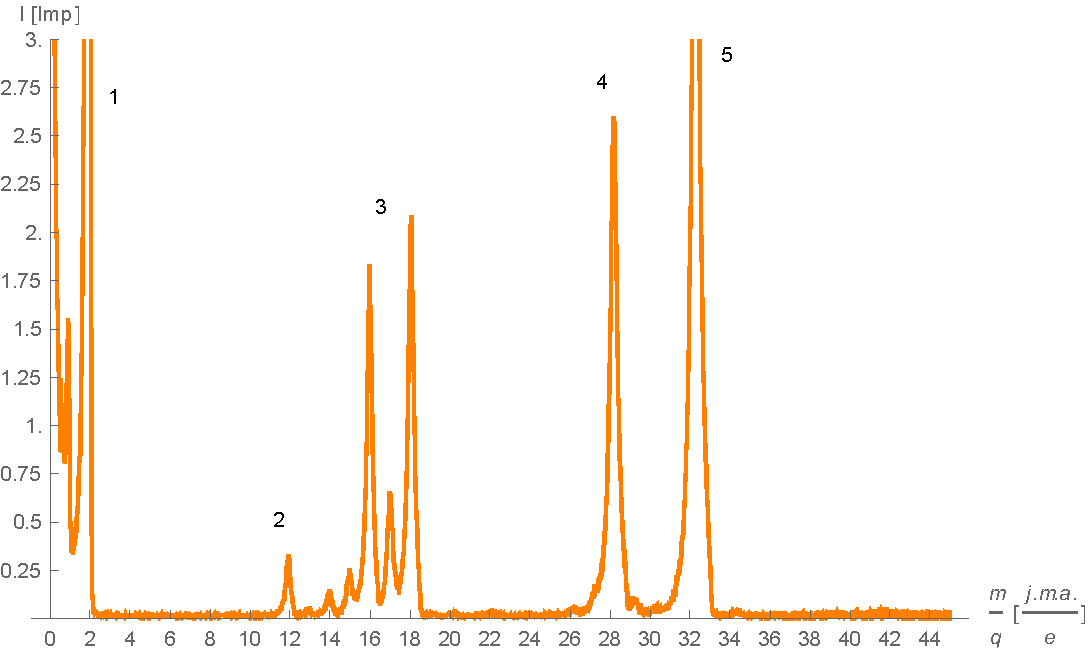
\includegraphics[width=0.7\linewidth]{spektlen}
\caption{Spektrum masowe po doprowadzeniu i ustabilizowaniu się poziomu tlenu.\newline 1 - peak elektrostatyczny(0-1) oraz wodór(2); 2 - węgiel(12); 3 - odpowiednio tlen(16),\newline tlenek wodoru(17) i woda(18); 4 - tlenek węgla(28); 5 - dwutlenek(32).}
\label{fig:spektlen}
\end{figure}

\section{Wnioski}
\subsection{Parametry i rodzielczość}
Dobrane przez nas parametry dają zadowalające wyniki przy akceptowalnym czasie pomiaru.\\
Rozdzielczość analizatora wynosi $d\alpha=0.8$. Biorąc pod uwagę, że wartości rzeczywiste stosunku masy oraz ładunku jonów i tak oscylują wokół wartości całkowitych, to rozdzielczość poniżej $1$ jest zadowalającą wartością. Jedyny problem może zaistnieć przy pomiarze zależności czasowej, który jest dokonywany dla konkretnych wartości tego stosunku.
\subsection{Gazy resztkowe}
Związki znajdujace się komorze próżniowej,to wodór, węgiel, tlen i azot. Są to związki zarówno występujące w atmosferze jak i w aparaturze. Jedynie zastanawiający jest azot, którego w odpowiednio odpompowanej aparaturze nie powinniśmy odnotowywać.
\subsection{Głowica Bayarda-Alperta}
Włączenie głowicy istotnie wpływa na skład chemiczny próżni. o może zmieniać wyniki pomiarów. Bo zapobiec temu, należy odpowiednio odgazowywać głowicę w ramach przygotowań do eksperymentów oraz umożliwić pompie jonowo-sorpyjnej odpompowanie gazów uwolnionych z głowicy, co wiąże się z pozostawieniem układu w spoczynku na dłuższy czas.
\subsection{Doprowadzenie tlenu do układu}
Wprowadzenie tlenu do układu zwiększa nie tylko stężenie cząstek $O_2$ i $O$, ale prowadzi do reakcji tlenu z wodorem, w wyniku czego w układzie pojawia się woda.
\begin{thebibliography}{99}

	\bibitem{grosz} J. Groszkowski, \emph{Technika wysokiej próżni}, Wydawnictwa Naukowo-Techniczne 1978 Warszawa
	\bibitem{podst} E. de Hoffmann, J. Charette, V. Stroobant, \emph{Spektrometria mas}, Wydawnictwa Naukowo-Techniczne, Warszawa 1998
	\bibitem{unipol} S. Mróz, E. Chrzanowski, \emph{Unipolarny filtr mas}, Wrocław 1974
	\bibitem{jonczyk} J. Jończyk, Projekt inżynierski: \emph{Sterowanie i akwizycja danych z unipolarnego filtru mas za pomocą przetownika National Instruments NI USB-6009}, Wrocław 2014
	
\end{thebibliography}
\end{document}